\documentclass{svproc}
%
% to typeset URLs, URIs, and DOIs
\usepackage{url}
\def\UrlFont{\rmfamily}
%
% Footnotes:
\usepackage[bottom]{footmisc}
%
% Images:
 \usepackage{graphicx}
%
\makeatletter
\newcommand{\verbatimfont}[1]{\renewcommand{\verbatim@font}{\ttfamily#1}}
\makeatother
%
\begin{document}
\mainmatter  % start of a contribution
\title{Reusing Conceptual Models:\newline Language and Extensible Compiler}
\titlerunning{Extensible Compiler for Conceptual Modeling}  % abbreviated title (for running head)
\toctitle{A Conceptual Modeling Language and Extensible Compiler} % used for the TOC 
\author{Quenio Cesar Machado dos Santos\inst{1} \and Raul Sidnei Wazlawick\inst{2}}
\authorrunning{Quenio C. M. dos Santos et al.} % abbreviated author list (for running head)
\tocauthor{Quenio Cesar Machado dos Santos, Raul Sidnei Wazlawick} % list of authors for the TOC
\institute{Computer Sciences,\\
UFSC - Universidade Federal de Santa Catarina, Brazil,\\
\email{queniodossantos@gmail.com}
\and
Associate Professor of Computer Sciences Department,\\
UFSC - Universidade Federal de Santa Catarina, Brazil,\\
 \email{raul@inf.ufsc.br}}

\maketitle              % typeset the title of the contribution

\begin{abstract}
This paper proposes a textual programming language
that enables conceptual modeling
(similarly to UML classes/associations and OCL constraints)
and a compiler that allows code generation
(via extensible textual templates)
to any target language or technology.
Together, the language and the compiler make it feasible
to specify (in a single high-level language)
the information of ever-changing, increasingly distributed software systems.
From this single source,
the automated code generation keeps the implementations 
(across the different platforms and technologies)
consistent with the specification.
Also, as the technology landscape evolves,
these textual models allow the recurring use of the investment made on their specification.
Unlike other approaches,
such as MDA and MPS,
the built-in tooling support,
along with the textual nature of this programming language and its extensible templates,
facilitates the integration to the workflow of software developers. 
\keywords{
conceptual modeling,
programming language,
code generation,
model-driven software development,
model-driven engineering, 
metaprogramming,
generative programming
}\end{abstract}

\section{Introduction}
%
In order to address the challenges of the ever-changing, increasingly distributed technologies used on software systems, the Model-Driven Architecture (MDA \cite{mda}) initiative by the Object Management Group (OMG) has been promoting model-driven software development.
In particular, MDA has guided the use of high-level models (created with OMG standards, such as UML \cite{uml}, OCL \cite{ocl} and MOF \cite{mof}) to derive software artifacts and implementations via automated transformations.
As one of its value propositions, the MDA guide \cite{mda} advocates:
\begin{quote}``Automation reduces the time and cost of realizing a design, reduces the time and cost for changes and maintenance and produces results that ensure consistency across all of the derived artifacts. For example, manually producing all of the web service artifacts required to implement a set of processes and services for an organization is difficult and error-prone. Producing execution artifacts from a model is more reliable and faster.''\end{quote} 

Even though MDA provides guidance and standards that can be used to realize its vision, it leaves to software vendors the task of providing the tools that automate the process of generating the implementations from the models.

The key role played by tools has been demonstrated by Voelter \cite{voelter} in his \emph{Generic Tools, Specific Languages} approach for model-driven software development. In his approach, Voelter \cite{voelter} has used domain-specific languages (DSL's) with the Metaprogramming System (MPS) in order to generate the software artifacts.
Unlike MDA, which is based on UML/MOF models, MPS allows the specification of models using domain-specific editors.
MPS itself is a generic tool, but it enables the definition of the abstract syntax, the editors and the code generators for DSL's.

The conceptual modeling language and extensible compiler presented here are an alternative approach to MPS.
While the latter is a fully integrated development environment based on domain-specific languages and their projectional editors, the former (hereby called CML) is a compiler that has:
\begin{itemize}
\item as \emph{input}, source files defined using its own conceptual language, which provides an abstract syntax similar to (but smaller than) a combination of UML \cite{uml} and OCL \cite{ocl}; 
\item and, as \emph{output}, any target languages based on extensible templates, which may be provided by the compiler's base library, by third-parties, or even by the developers themselves.
\end{itemize}

\section{Why A New Language?}\label{sec:why}

Thalheim \cite{thalheim} has observed that
the choice of a conceptual modeling language has to do with its purpose.
He suggests that
a language is just a \emph{carrier} mapping some properties of the \emph{origin} (the problem space)
that can provide utility to its users. 

In this context, the purpose of the CML language is being a tool
that allows software developers to transform text-based conceptual models
into executable code of an extensible range of technologies.
In order to achieve this purpose,
a new language is designed with the high-level goals presented in the following subsections.

\subsection{Developer Experience}

CML follows the principle laid out on the \emph{Conceptual-Model Programming} (CMP) manifesto \cite{cmp}:

\begin{quote}
``Conceptual modeling is programming.
The conceptual-model instance is the code,
i.e., instead of `the code is the model,'
the phrase now becomes `the model is the code.'
A conceptual-model compiler assures that program execution corresponds to the conceptual specification,
thus making the conceptual-model instance directly executable.''
\end{quote}

Furthermore,
CML is also intended to enable software developers to do \emph{conceptual modeling} on the same workflow they are used to doing \emph{programming}.
CML strives to \emph{not only be} the code (as advocated by CMP),
but also \emph{look like} code (syntactically speaking),
pursuing compatibility with developers' mindset, toolset and workflow.
By providing its own syntax based on existing programming languages,
CML then promotes the \emph{modeling-as-programming} approach. 

The UML \cite{uml} notation, on the other hand,
being graphical,
is not suited for mainstream, textual programming.
However, the \emph{Human Usable Textual Notation} (HUTN) \cite{hutn} is a textual syntax for MOF-based \cite{mof} metamodels,
and as such, it can also be used for UML models.
The syntax of the structural (static) elements of CML models is based on HUTN.

The OWL 2 standard, as another example, provides the Manchester \cite{owl2manchester} syntax,
which is intended to be user-friendly.
However, it does not resemble the syntax of commonly used, block-based, imperative programming languages,
such as C \cite{clang} and its syntax-alike descendants.
Manchester's syntax is also unlike the syntax of declarative, query languages, such as SQL \cite{sql}.

Using CML,
and its familiar syntax (as we shall demonstrate in the next sections),
it is expected that developers can raise the abstraction level of their programs.

\subsection{Language Evolution}

CML is expected to evolve with its compiler, and the tooling around it.
Unlike the expressive power seen on UML \cite{uml} and OWL 2 \cite{owl2} with their breadth of features,
the CML language and its extensible compiler intentionally support a limited number of features and scenarios.

This first version has been designed for the initial validation of the model-driven development approach taken by CML.
As developers provide feedback,
new language features may be iteratively added in order to enable the extensible CML compiler to support new modeling/development scenarios.

\subsection{Extensible Target Generation}

Some of the language features enable the generation of code into a wide range of target languages and technologies. Among the features that must be provided by the CML language, there is the ability to:

\begin{itemize}
\item break models into modules that can be shared as libraries;
\item specify different code generation targets;
\item and annotate model elements in order to provide more information for specific targets during code generation.
\end{itemize}

These features need to be available in a single language, they have to compatible with each other and with the code generation backend.


\section{The Language}\label{sec:lang}
%
This section presents an overview of the conceptual modeling language.
The \emph{concrete syntax} is presented using an example in subsection \ref{subsec:example}.
The mapping of the CML example to other modeling notations is illustrated in subsection \ref{subsec:mapping}.
The CML metamodel (the \emph{abstract syntax}'s structure) is presented in subsection \ref{subsec:metamodel}.
(The \emph{CML specification} \cite{cml-spec} provides a formal description of the \emph{concrete syntax},
along with its mapping to the \emph{abstract syntax}.)

\subsection{An Example}\label{subsec:example}

On the example of figure \ref{fig:store}, some concepts, such as \emph{Book} and \emph{Customer}, are declared in CML.
The block-based syntax declaring each concept resembles the C \cite{clang} language's syntax.
Each concept declares a list of properties.
The property declarations are based on the Pascal \cite{pascal} style for variable declarations,
where the name is followed by a colon (``:'') and then the type declaration.
Part of the CML syntax for expressions, such as the expression in \emph{BookStore}'s \emph{orderedBooks}, is based on OCL \cite{ocl} expressions; while the syntax of the expression in \emph{goldCustomers} is new, its semantics also match OCL \cite{ocl} query expressions.

\begin{figure}
\verbatimfont{\small}
\begin{verbatim}
concept BookStore
{
    books: Book+;
    customers: Customer*;
    orders: Order*;
    /goldCustomers = customers | select totalSales > 1000;
    /orderedBooks = orders.items.book;
}

concept Book
{
    title: String;
    price: Decimal;
    quantity: Integer = 0;
}

concept Customer
{
    orders: Order*;
    /totalSales = orders | collect result += total;
}

concept Order
{
    customer: Customer;
    total: Decimal;
}

association CustomerOrder
{
    Order.customer: Customer;
    Customer.orders: Order*;
}
\end{verbatim}
\caption{The example above is adapted to CML from the fictional Livir bookstore, which is presented as a case study in Wazlawick \cite{wazlawick}.}
\label{fig:store}
\end{figure}


The key language features are:
\emph{Book} and \emph{Customer} are concepts;
\emph{title} and \emph{price} under the \emph{Book} concept are attributes;
\emph{totalSales} under the \emph{Customer} concept is a derived attribute;
the \emph{books} and \emph{customers} properties declared under the \emph{BookStore} concept represent unidirectional associations (in UML \cite{uml}, they would correspond to the association roles);
\emph{CustomerOrder} binds two unidirectional associations
(represented by the \emph{orders} property under the \emph{Customer} concept
and by the \emph{customer} property under the \emph{Order} concept)
into a single bidirectional association;
the \emph{goldCustomers} and \emph{orderedBooks} properties under the \emph{BookStore} concept are examples of derived associations. These language features will be defined in the subsection \ref{subsec:metamodel}.

\subsection{Mapping CML Source to UML and OCL}\label{subsec:mapping}

Part of the CML metamodel (presented in section \ref{subsec:metamodel})
may be considered a small subset of the UML  \cite{uml} metamodel.
Thus, the structural (static) elements of CML models can be transformed into UML class diagrams.
The example CML model in the listing of figure \ref{fig:store} is mapped to the UML model in figure \ref{fig:uml}.

\begin{figure}
\centering
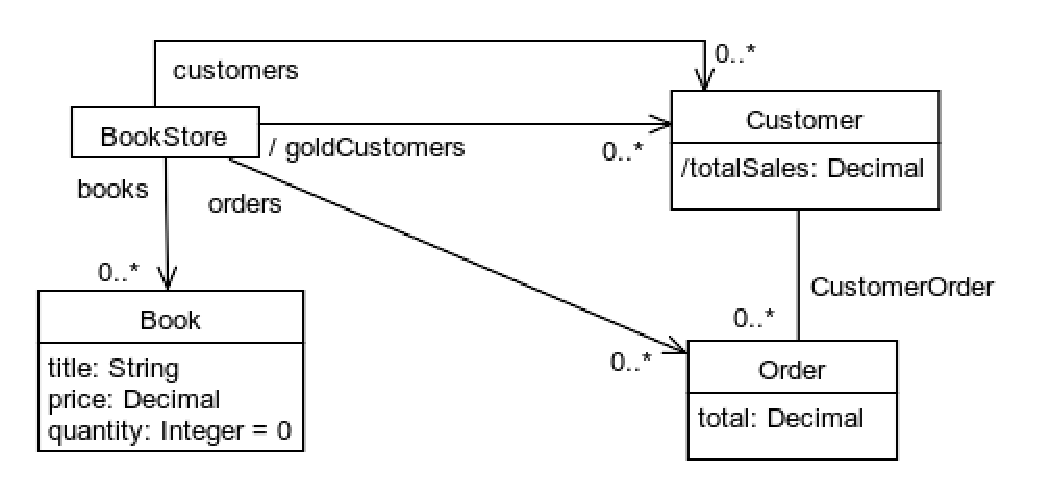
\includegraphics[width=0.8\textwidth]{language/diagram-uml}
\caption{The UML class diagram \cite{uml} for the CML model listed in figure \ref{fig:store}.}
\label{fig:uml}
\end{figure}

In figure \ref{fig:uml},
the CML concepts (\emph{BookStore}, \emph{Book}, \emph{Customer} and \emph{Order})
are mapped to corresponding UML classes.
The CML properties that represent attributes
(such as \emph{title}, \emph{quantity} and \emph{price} of \emph{Book})
are mapped to UML attributes under each class.
The CML properties that represent unidirectional associations
(\emph{books}, \emph{customers}, and \emph{goldCustomers} of \emph{BookStore})
are mapped to UML associations with corresponding roles
(showing the navigability direction, and matching the property names and cardinality.)
The CML bidirectional association \emph{CustomerOrder}
(comprised by two CML properties: \emph{Customer.orders} and \emph{Order.customer})
is mapped to a UML association with bidirectional navigability (that is, no direction arrow.)
As demonstrated by this example,
CML strives to enable modeling at the same conceptual level as allowed by UML.
That being said, when compared to the UML metamodel,
the CML metamodel supports only a core set of its elements,
as shown in subsection \ref{subsec:metamodel}.

Besides the structural elements of a conceptual model (as seen above),
CML also has expressions that can set initial values to attributes,
and define derived properties for both attributes and associations.
CML expressions are partially based on the OCL \cite{ocl} syntax,
but they follow closely the OCL semantics.
For example,
the following CML expression (extracted from figure \ref{fig:store}) is
a path-based navigation expression borrowed from OCL:

\verbatimfont{\small}
\begin{verbatim}
/orderedBooks = orders.items.book;
\end{verbatim}

Using association properties,
the expression above navigates from one instance of \emph{BookStore},
passing through all linked \emph{orders},
and then through all \emph{items} of all \emph{orders},
in order to return all books that have been ordered.
As another example, the following CML expression
(also extracted from figure \ref{fig:store}) does not follow the OCL syntax:

\verbatimfont{\small}
\begin{verbatim}
/goldCustomers = customers | select: totalSales > 1000;
\end{verbatim}

However, the expression above closely matches the semantics of the following OCL expression:

\verbatimfont{\small}
\begin{verbatim}
derive: customers->select(totalSales > 1000)
\end{verbatim}

Both the CML expression and the OCL excerpt above evaluate to a set of \emph{Customer} instances
that have bought more than 1000 in the \emph{BookStore}.

The OCL syntax for expressions that process collections of instances has the following general form:

\verbatimfont{\small}
\begin{verbatim}
collection->method_name(predicate or function)
\end{verbatim}

The expression above is based on method invocations
(an influence from UML's object-oriented paradigm),
and thus it has an imperative style.
CML, on the other hand, intends to be agnostic towards programming paradigms.
By using extensible comprehensions \cite{trinder}
to define derived attributes and associations,
CML's syntax is more declarative,
similar to SQL \cite{sql} or C\#'s LINQ \cite{torgersen}.
In CML, smaller expressions can also be combined into larger ones. For example:

\verbatimfont{\small}
\begin{verbatim}
/goldOrders = for order in bookStore.orders,
                  goldCustomer in bookStore.goldCustomers
                  | select: order.customer == goldCustomer | yield: order
 \end{verbatim}

Above, all \emph{orders} from \emph{goldCustomers} are returned.
The sub-expressions are evaluated sequentially:
the \emph{for} expression provides a cross join of all (\emph{order}, \emph{goldCustomer}) pairs;
the \emph{select} expression selects only the pairs that have matching customers;
Finally, the \emph{yield} expression maps selected pairs into a sequence of \emph{orders}.
Sub-expressions like \emph{for}, \emph{select} and \emph{yield} can be combined in different configurations
in order to derive any required attributes and associations.

\subsection{The CML Metamodel (Abstract Syntax)}\label{subsec:metamodel}

In the article \emph{UML and OCL in Conceptual Modeling}, 
Gogolla \cite{gogolla} shows, by mapping the UML \cite{uml} metamodel to the ER \cite{er} metamodel,
how UML models (augmented by OCL \cite{ocl} constraints) can be used to specify conceptual models.
Also, Wazlawick \cite{wazlawick} systematically prescribes in his book a method for conceptual modeling using UML and OCL. 

Since one key CML goal is enabling the specification of conceptual models
(such as those specified by ER models and UML/OCL models),
in order to present the key elements of the CML metamodel,
a similar approach to Gogolla's is used to map the CML metamodel to the ER metamodel,
and to the UML/OCL metamodel.

\pagebreak[4]

The EMOF \cite{mof} model presented by figure \ref{fig:metamodel} is a simplified version of the CML metamodel:

\begin{figure}
\centering
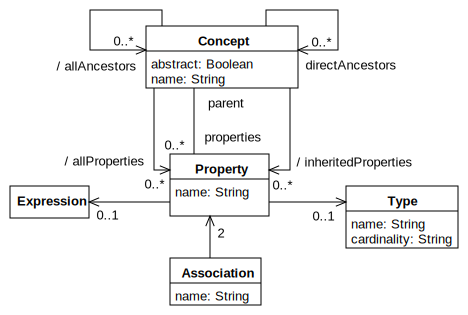
\includegraphics[width=0.8\textwidth]{language/diagram-metamodel}
\caption{This class diagram renders the EMOF \cite{mof} model defining the CML metamodel.}
\label{fig:metamodel}
\end{figure}

In CML metamodel shown in figure \ref{fig:metamodel},
a \emph{Concept} is composed of zero-or-more \emph{Property} instances.
Each \emph{Property} may have a \emph{Type} and an \emph{Expression}.
If two \emph{Property} instances represent the same bidirectional association,
there must be an \emph{Association} instance that binds them.
Unidirectional associations are only represented by the \emph{Property} instance (representing the association role)
that enables the navigation from the source \emph{Concept} instance to the target one (which is represented by the property's \emph{Type}.)

Next, there is a description for the key metamodel elements.

\subsubsection{Concept.}

According to Wazlawick \cite{wazlawick},
a concept represents complex information that has a coherent meaning in the domain.
They aggregate attributes and cannot be described as primitive values.
They may also be associated with other concepts.
On the ER metamodel, it is known as \emph{entity};
on the UML metamodel, as \emph{class}.

\subsubsection{Property.}

May be an attribute holding values of primitive types,
or references (or collections of references) linking concepts.
On the ER metamodel,
the set of all references is known as \emph{relationship};
on the UML metamodel, unidirectional associations.
Attributes have the same name on all metamodels.

\subsubsection{Association.}

Unlike the ER and UML metamodels, in the CML metamodel, only bidirectional associations are represented with the Association class. They bind the non-primitive properties (from the same or from different concepts.) 


\subsubsection{Type.} They may be primitive types (such as Boolean, String, Decimal, and Regex), references to concept instances, or still collections of concepts. They may also be optional, meaning their value may or may not have been set.


\section{The Extensible Compiler}\label{sec:compiler}

In order to realize the CMP \cite{cmp} manifesto's vision,
the CML compiler generates code in any target language based on extensible templates.
A set of core templates is provided by the CML compiler's base libraries.
Third-party libraries can also provide their own templates,
along with their conceptual models,
in order to target specific technologies or platforms.
Developers can also extend existing templates in order to adapt the implementation to characteristics specific to their projects.

Subsection \ref{subsec:overview} will provide an overview of the CML compiler's architecture.
Next, subsection \ref{subsec:templates} will introduce the CML compiler's extensible templates.
Finally, subsection \ref{subsec:modlib} will lay out the CML compiler's mechanism for organizing and sharing conceptual models and extensible templates.

\subsection{Compiler Overview}\label{subsec:overview}

An overview diagram of the architecture is shown in figure \ref{fig:overview}.

\begin{figure}
\centering
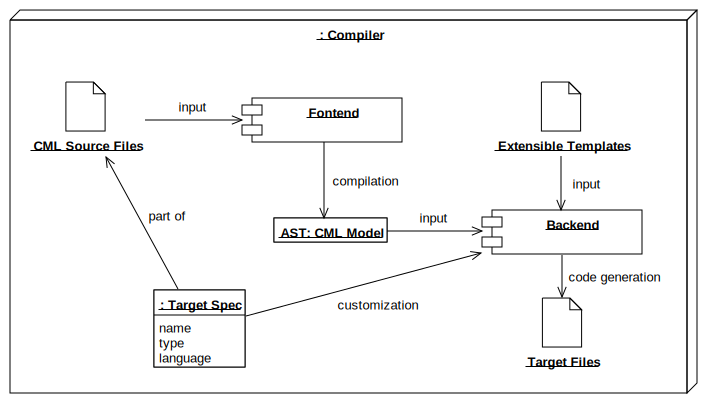
\includegraphics[width=0.7\textwidth]{compiler/figure-overview}
\caption{An architectural overview of the CML compiler.}
\label{fig:overview}
\end{figure}

The two main components of the compiler,
and the artifacts they work with,
are presented below:

\begin{itemize}

\item \emph{Frontend:} receives as input the \emph{CML source files}.
It will parse the files and generate an internal representation of the \emph{CML model}.
Syntactical and semantic validations will be executed at this point.
Any errors are presented to the developer, interrupting the progress to the next phase.
If the \emph{source files} are parsed and validated successfully, then an internal representation (AST) of the \emph{CML model} is generated, as shown in subsection \ref{subsec:ast}.
The AST serves then as the input for the \emph{backend} component.

\item \emph{Backend:} receives the \emph{CML model AST} as input.
Based on the \emph{target specification} provided by the AST, chooses which \emph{extensible templates} to use for code generation.
The \emph{target files} are then generated, and become available to be consumed by other tools. The \emph{target specification} plays a key role in order to determine the kind of \emph{target} to be generated, and it is presented in subsection \ref{subsec:templates}.

\end{itemize}

\subsection{Extensible Templates}\label{subsec:templates}

Parr has formalized and developed the StringTemplate \cite{st} language for code generation. CML extensible templates are implemented in StringTemplate. The CML compiler uses StringTemplate for two purposes:

\begin{itemize}

\item \emph{File names and directory structure:}
each type of target generated by the CML compiler requires a different directory structure.
The CML compiler expects each target type to define a template file named ``files.stg'' (also known as \emph{files template}),
which will contain the path of all files to be generated.
The \emph{files template} may use information provided by the \emph{target specification} (introduced in subsection \ref{subsec:overview})
in order to determine the file/directory names.
An example of a \emph{files template} is shown below:
\verbatimfont{\scriptsize}
\begin{verbatim}
moduleFiles(target, module) ::= <<
maven:pom|pom.xml
>>

conceptFiles(target, concept) ::= <<
dto|src/main/java/<target.packagePath>/<concept.name>.java
>>
\end{verbatim}

\item \emph{File content generation:}
each file listed under the \emph{files template} will have a corresponding \emph{content template} that specifies how the file's content must be generated. The \emph{content template} will receive as input one root-level element of the CML model, which will provide information to generate the file's content. The type of model element received as input by the \emph{content template} depends on which function of the \emph{files template} has defined the file to be generated.
A typical \emph{content template} is shown below:
\verbatimfont{\scriptsize}
\begin{verbatim}
import "/lang/class.stg"

dto(target, concept) ::= <<
package <target.packageName>;

import java.util.*;

public <class(concept)>
>>
\end{verbatim}


\end{itemize}

On the \emph{files template} example,
two types of files are created for this target:
one file for the CML module (named ``pom.xml'', and based on the ``pom'' template); and one for each concept found in the CML model (with the file extension ``.java'', and based on the ``dto'' template.)

On the \emph{content template} example, the ``dto'' content template is displayed, which can generate a \emph{Data Type Object} (DTO) class in Java. The actual template that knows how to generate the class is imported from ``/lang/class.stg''.

\subsection{Modules and Libraries}\label{subsec:modlib}

When developing a single application with just a few targets, having a single directory to maintain all the CML source code is sufficient. But, once more than one application is developed as part of a larger project, and CML model elements are shared among them, it is necessary to separate the common source code. Also, some applications cover different domains, and it may be beneficial to separate the source code into different CML models.

In order to allow that, CML supports \emph{modules}. Grouping a set of CML model elements, a module in CML is conceptually similar to a UML \cite{uml} package. Physically, each module is a directory containing three sub-directories:

\begin{itemize}
\item \emph{source}: where the CML source files reside.
\item \emph{templates}: optional directory containing templates for code generation.
\item \emph{targets}: created by the CML compiler to contain each target sub-directory, which in turn contains the target files generated for a given target.
\end{itemize}

Under the \emph{source} directory, the module is defined by a \emph{module specification}. If a module needs to reference CML model elements in other modules, then an import statement defines the name of the other modules. The CML compiler will then compile the imported modules before compiling the current module.

In order for the CML compiler to find the other modules, they must be in a sub-directory with the module's name in the same directory where the current module is placed.

CML modules have no versions as they are maintained in the same code repository with the other modules they import. However, one can package a module as a library, which will have a version and the same name as the module. This library in turn can be published into a public (or company-wide) \emph{library site} in order to be shared with other developers.

A CML library is just a packaged, read-only module with a version of the format: 

\verbatimfont{\small}
\begin{verbatim}
revision[.accretion][.fix]
\end{verbatim}

Where semantic versioning \cite{semver} is followed:
\begin{itemize}
\item \emph{revision} is the number of a library release incompatible with any previous releases with a lower revision number.
\item \emph{accretion} is the number of a library release compatible with any previous accretion number of the same revision.
\item \emph{fix} is the number of a library release that fixes an issue in a previous accretion.
\end{itemize}

Compatible versions do not change or remove public elements of the library's CML model (or function/parameters from the library's templates); only add new elements. Fixes cannot change the library's public elements; only internal elements. These rules may be enforced by the CML compiler when packaging and publishing new versions of a library.


\section{Related Work}\label{sec:related}

The following subsections compare CML to other languages, tools and frameworks
that can also generate code from conceptual models.
Each subsection covers a different category,
enumerating specific solutions and characterizing their relevance to CML, and also their differences. 

\subsection{Textual Languages}

This subsection covers existing text-based languages designed to enable code generation from conceptual models.
When compared to CML, the following languages are the most relevant,
because they are all textual languages designed for code generation:

\begin{itemize}
\item MPS \cite{voelter}
\item Xtext/Xtend
\item M Language
\item MM-DSL
\item XML/XSLT
\item IFML
\end{itemize}

Observe that most of the solutions listed above enable modeling via DSLs, while CML is a generic language for modeling in any domain.

\subsection{Graphical Languages}

This subsection covers existing graphical languages designed to enable code generation from conceptual models.
Despite CML being a textual language,
the following graphical languages still have some relevance,
because they have also been used to generate code in other target languages:

\begin{itemize}
\item MPS \cite{voelter}
\item FCML \cite{fcml}
\item MetaEdit+ \cite{metaedit}
\item MDA \cite{mda}
\end{itemize}

The major drawback behind graphical languages,
as covered in section \ref{sec:why},
is their difficulty to integrate seamlessly with the workflow, tools and mindset of software developers.

\subsection{Frameworks}

Frameworks allow code generation from conceptual models, but lack a modeling language -- graphical or textual. 
EMF is a classical example,
where modeling is done via editors on Eclipse or via a programming interface,
and the models are stored in the ECORE/XML format. 

Frameworks may also be used as the infrastructure of modeling languages.
EMF, for example, is the framework supporting Xtext.
Conceivably, other modeling languages may also target EMF.
In fact, CML's extensible compiler allows the implementation of templates that target EMF.

\subsection{Template Languages}

As seen in previous sections,
the CML compiler uses StringTemplate as the language for its code generation templates.
There are other template languages designed for code generation from conceptual models:

\begin{itemize}
\item Xpand \cite{xpand}
\item EGL \cite{egl}
\item MOFScript \cite{mofscript}
\item JET \cite{jet}
\end{itemize}

One major strength of StringTemplate over the options above is its extensibility mechanisms.
It is possible to define a core set of templates that define patterns, 
and then extend them with the specifics of each target language or technology.
It is also possible to share templates as libraries,
which can be further extended for specific purposes by third-parties.

\subsection{Languages Supporting Associations}

Just as CML,
and unlike most programming languages,
there are a number of languages that provide the ability to declare bidirectional associations:

\begin{itemize}
\item ASSOCIATION\# \cite{cardoso}
\item DSM \cite{balzer}
\item RelJ \cite{bierman}
\item Fibonacci \cite{fibonacci}
\end{itemize}

One key drawback of the languages listed above is the fact that their conceptual models
cannot be reused to generate code in any other language or technology;
they are, for all intents and purposes, the target language.

\subsection{Other Languages}

There are also other conceptual languages whose original focus has not been to support code generation or implementation,
but to serve solely as modeling artifacts.

Languages, such as OWL and Telos, have been designed as ontology metamodels
to support the representation and storage of knowledge,
and to allow automated reasoning from knowledgebases.
OWL being the \emph{lingua franca} of the semantic web,
while Telos has been created to store ontologies in a object-oriented database.
Other languages, like UML and ER, have been originally intended as tools to support the analysis and design of software systems, and only after sometime have been repurposed for model-driven software development.

The relevance of these languages to CML comes from the expressivity power their metamodels provide for conceptual modeling. For that reason, when convenience and appropriate, CML should remain to expand its capabilities by borrowing features from these languages.

\section{Conclusion}\label{sec:conclusion}

The CML language and compiler make it possible to specify,
in a single high-level language,
the concepts of ever-changing, increasingly distributed software systems.

As opposed to implementing these concepts, their properties and associations in each target language,
from a single CML model,
the CML extensible templates generate code that
keeps the implementations 
(across the different platforms and technologies) 
consistent with the specification.
Also, as the technology landscape evolves,
these textual CML models can be reused to generate code in new target languages and technologies.

The initial version of CML has been designed to validate this textual, model-driven approach of development.
Practical application of CML in software development is needed in order to provide qualitative evidence that
CML can indeed be used as a single source to implement multiple targets.
Quantitative cost-benefit analysis
(based on the implementation effort of hand-written vs generated lines-of-code, perhaps using a method adapted from the work of Gaffney et al \cite{gaffney})
may also provide data
that shows whether the investment -- made on the development of CML models -- pays off. The data collected, together with the feedback provided by software developers, should then inform the iterative design of new CML features.

%
\bibliographystyle{spmpsci}
\bibliography{references}
%
\end{document}
